% Options for packages loaded elsewhere
\PassOptionsToPackage{unicode}{hyperref}
\PassOptionsToPackage{hyphens}{url}
\PassOptionsToPackage{dvipsnames,svgnames,x11names}{xcolor}
%
\documentclass[
  letterpaper,
  DIV=11,
  numbers=noendperiod]{scrartcl}

\usepackage{amsmath,amssymb}
\usepackage{iftex}
\ifPDFTeX
  \usepackage[T1]{fontenc}
  \usepackage[utf8]{inputenc}
  \usepackage{textcomp} % provide euro and other symbols
\else % if luatex or xetex
  \usepackage{unicode-math}
  \defaultfontfeatures{Scale=MatchLowercase}
  \defaultfontfeatures[\rmfamily]{Ligatures=TeX,Scale=1}
\fi
\usepackage{lmodern}
\ifPDFTeX\else  
    % xetex/luatex font selection
\fi
% Use upquote if available, for straight quotes in verbatim environments
\IfFileExists{upquote.sty}{\usepackage{upquote}}{}
\IfFileExists{microtype.sty}{% use microtype if available
  \usepackage[]{microtype}
  \UseMicrotypeSet[protrusion]{basicmath} % disable protrusion for tt fonts
}{}
\makeatletter
\@ifundefined{KOMAClassName}{% if non-KOMA class
  \IfFileExists{parskip.sty}{%
    \usepackage{parskip}
  }{% else
    \setlength{\parindent}{0pt}
    \setlength{\parskip}{6pt plus 2pt minus 1pt}}
}{% if KOMA class
  \KOMAoptions{parskip=half}}
\makeatother
\usepackage{xcolor}
\setlength{\emergencystretch}{3em} % prevent overfull lines
\setcounter{secnumdepth}{-\maxdimen} % remove section numbering
% Make \paragraph and \subparagraph free-standing
\makeatletter
\ifx\paragraph\undefined\else
  \let\oldparagraph\paragraph
  \renewcommand{\paragraph}{
    \@ifstar
      \xxxParagraphStar
      \xxxParagraphNoStar
  }
  \newcommand{\xxxParagraphStar}[1]{\oldparagraph*{#1}\mbox{}}
  \newcommand{\xxxParagraphNoStar}[1]{\oldparagraph{#1}\mbox{}}
\fi
\ifx\subparagraph\undefined\else
  \let\oldsubparagraph\subparagraph
  \renewcommand{\subparagraph}{
    \@ifstar
      \xxxSubParagraphStar
      \xxxSubParagraphNoStar
  }
  \newcommand{\xxxSubParagraphStar}[1]{\oldsubparagraph*{#1}\mbox{}}
  \newcommand{\xxxSubParagraphNoStar}[1]{\oldsubparagraph{#1}\mbox{}}
\fi
\makeatother

\usepackage{color}
\usepackage{fancyvrb}
\newcommand{\VerbBar}{|}
\newcommand{\VERB}{\Verb[commandchars=\\\{\}]}
\DefineVerbatimEnvironment{Highlighting}{Verbatim}{commandchars=\\\{\}}
% Add ',fontsize=\small' for more characters per line
\usepackage{framed}
\definecolor{shadecolor}{RGB}{241,243,245}
\newenvironment{Shaded}{\begin{snugshade}}{\end{snugshade}}
\newcommand{\AlertTok}[1]{\textcolor[rgb]{0.68,0.00,0.00}{#1}}
\newcommand{\AnnotationTok}[1]{\textcolor[rgb]{0.37,0.37,0.37}{#1}}
\newcommand{\AttributeTok}[1]{\textcolor[rgb]{0.40,0.45,0.13}{#1}}
\newcommand{\BaseNTok}[1]{\textcolor[rgb]{0.68,0.00,0.00}{#1}}
\newcommand{\BuiltInTok}[1]{\textcolor[rgb]{0.00,0.23,0.31}{#1}}
\newcommand{\CharTok}[1]{\textcolor[rgb]{0.13,0.47,0.30}{#1}}
\newcommand{\CommentTok}[1]{\textcolor[rgb]{0.37,0.37,0.37}{#1}}
\newcommand{\CommentVarTok}[1]{\textcolor[rgb]{0.37,0.37,0.37}{\textit{#1}}}
\newcommand{\ConstantTok}[1]{\textcolor[rgb]{0.56,0.35,0.01}{#1}}
\newcommand{\ControlFlowTok}[1]{\textcolor[rgb]{0.00,0.23,0.31}{\textbf{#1}}}
\newcommand{\DataTypeTok}[1]{\textcolor[rgb]{0.68,0.00,0.00}{#1}}
\newcommand{\DecValTok}[1]{\textcolor[rgb]{0.68,0.00,0.00}{#1}}
\newcommand{\DocumentationTok}[1]{\textcolor[rgb]{0.37,0.37,0.37}{\textit{#1}}}
\newcommand{\ErrorTok}[1]{\textcolor[rgb]{0.68,0.00,0.00}{#1}}
\newcommand{\ExtensionTok}[1]{\textcolor[rgb]{0.00,0.23,0.31}{#1}}
\newcommand{\FloatTok}[1]{\textcolor[rgb]{0.68,0.00,0.00}{#1}}
\newcommand{\FunctionTok}[1]{\textcolor[rgb]{0.28,0.35,0.67}{#1}}
\newcommand{\ImportTok}[1]{\textcolor[rgb]{0.00,0.46,0.62}{#1}}
\newcommand{\InformationTok}[1]{\textcolor[rgb]{0.37,0.37,0.37}{#1}}
\newcommand{\KeywordTok}[1]{\textcolor[rgb]{0.00,0.23,0.31}{\textbf{#1}}}
\newcommand{\NormalTok}[1]{\textcolor[rgb]{0.00,0.23,0.31}{#1}}
\newcommand{\OperatorTok}[1]{\textcolor[rgb]{0.37,0.37,0.37}{#1}}
\newcommand{\OtherTok}[1]{\textcolor[rgb]{0.00,0.23,0.31}{#1}}
\newcommand{\PreprocessorTok}[1]{\textcolor[rgb]{0.68,0.00,0.00}{#1}}
\newcommand{\RegionMarkerTok}[1]{\textcolor[rgb]{0.00,0.23,0.31}{#1}}
\newcommand{\SpecialCharTok}[1]{\textcolor[rgb]{0.37,0.37,0.37}{#1}}
\newcommand{\SpecialStringTok}[1]{\textcolor[rgb]{0.13,0.47,0.30}{#1}}
\newcommand{\StringTok}[1]{\textcolor[rgb]{0.13,0.47,0.30}{#1}}
\newcommand{\VariableTok}[1]{\textcolor[rgb]{0.07,0.07,0.07}{#1}}
\newcommand{\VerbatimStringTok}[1]{\textcolor[rgb]{0.13,0.47,0.30}{#1}}
\newcommand{\WarningTok}[1]{\textcolor[rgb]{0.37,0.37,0.37}{\textit{#1}}}

\providecommand{\tightlist}{%
  \setlength{\itemsep}{0pt}\setlength{\parskip}{0pt}}\usepackage{longtable,booktabs,array}
\usepackage{calc} % for calculating minipage widths
% Correct order of tables after \paragraph or \subparagraph
\usepackage{etoolbox}
\makeatletter
\patchcmd\longtable{\par}{\if@noskipsec\mbox{}\fi\par}{}{}
\makeatother
% Allow footnotes in longtable head/foot
\IfFileExists{footnotehyper.sty}{\usepackage{footnotehyper}}{\usepackage{footnote}}
\makesavenoteenv{longtable}
\usepackage{graphicx}
\makeatletter
\def\maxwidth{\ifdim\Gin@nat@width>\linewidth\linewidth\else\Gin@nat@width\fi}
\def\maxheight{\ifdim\Gin@nat@height>\textheight\textheight\else\Gin@nat@height\fi}
\makeatother
% Scale images if necessary, so that they will not overflow the page
% margins by default, and it is still possible to overwrite the defaults
% using explicit options in \includegraphics[width, height, ...]{}
\setkeys{Gin}{width=\maxwidth,height=\maxheight,keepaspectratio}
% Set default figure placement to htbp
\makeatletter
\def\fps@figure{htbp}
\makeatother

\usepackage{booktabs}
\usepackage{longtable}
\usepackage{array}
\usepackage{multirow}
\usepackage{wrapfig}
\usepackage{float}
\usepackage{colortbl}
\usepackage{pdflscape}
\usepackage{tabu}
\usepackage{threeparttable}
\usepackage{threeparttablex}
\usepackage[normalem]{ulem}
\usepackage{makecell}
\usepackage{xcolor}
\KOMAoption{captions}{tableheading}
\makeatletter
\@ifpackageloaded{caption}{}{\usepackage{caption}}
\AtBeginDocument{%
\ifdefined\contentsname
  \renewcommand*\contentsname{Table of contents}
\else
  \newcommand\contentsname{Table of contents}
\fi
\ifdefined\listfigurename
  \renewcommand*\listfigurename{List of Figures}
\else
  \newcommand\listfigurename{List of Figures}
\fi
\ifdefined\listtablename
  \renewcommand*\listtablename{List of Tables}
\else
  \newcommand\listtablename{List of Tables}
\fi
\ifdefined\figurename
  \renewcommand*\figurename{Figure}
\else
  \newcommand\figurename{Figure}
\fi
\ifdefined\tablename
  \renewcommand*\tablename{Table}
\else
  \newcommand\tablename{Table}
\fi
}
\@ifpackageloaded{float}{}{\usepackage{float}}
\floatstyle{ruled}
\@ifundefined{c@chapter}{\newfloat{codelisting}{h}{lop}}{\newfloat{codelisting}{h}{lop}[chapter]}
\floatname{codelisting}{Listing}
\newcommand*\listoflistings{\listof{codelisting}{List of Listings}}
\makeatother
\makeatletter
\makeatother
\makeatletter
\@ifpackageloaded{caption}{}{\usepackage{caption}}
\@ifpackageloaded{subcaption}{}{\usepackage{subcaption}}
\makeatother
\ifLuaTeX
  \usepackage{selnolig}  % disable illegal ligatures
\fi
\usepackage{bookmark}

\IfFileExists{xurl.sty}{\usepackage{xurl}}{} % add URL line breaks if available
\urlstyle{same} % disable monospaced font for URLs
\hypersetup{
  pdftitle={Namibian hake model update, 2024},
  pdfauthor={John Kathena, Jim Ianelli},
  colorlinks=true,
  linkcolor={blue},
  filecolor={Maroon},
  citecolor={Blue},
  urlcolor={Blue},
  pdfcreator={LaTeX via pandoc}}

\title{Namibian hake model update, 2024}
\author{John Kathena, Jim Ianelli}
\date{2024-07-16}

\begin{document}
\maketitle

\renewcommand*\contentsname{Contents}
{
\hypersetup{linkcolor=}
\setcounter{tocdepth}{3}
\tableofcontents
}
\begin{Shaded}
\begin{Highlighting}[]
\FunctionTok{library}\NormalTok{(knitr)}
\NormalTok{hook\_output }\OtherTok{=}\NormalTok{ knit\_hooks}\SpecialCharTok{$}\FunctionTok{get}\NormalTok{(}\StringTok{\textquotesingle{}output\textquotesingle{}}\NormalTok{)}
\NormalTok{knit\_hooks}\SpecialCharTok{$}\FunctionTok{set}\NormalTok{(}\AttributeTok{output =} \ControlFlowTok{function}\NormalTok{(x, options) \{}
  \CommentTok{\# this hook is used only when the linewidth option is not NULL}
  \ControlFlowTok{if}\NormalTok{ (}\SpecialCharTok{!}\FunctionTok{is.null}\NormalTok{(n }\OtherTok{\textless{}{-}}\NormalTok{ options}\SpecialCharTok{$}\NormalTok{linewidth)) \{}
\NormalTok{    x }\OtherTok{=}\NormalTok{ knitr}\SpecialCharTok{:::}\FunctionTok{split\_lines}\NormalTok{(x)}
    \CommentTok{\# any lines wider than n should be wrapped}
    \ControlFlowTok{if}\NormalTok{ (}\FunctionTok{any}\NormalTok{(}\FunctionTok{nchar}\NormalTok{(x) }\SpecialCharTok{\textgreater{}}\NormalTok{ n)) x }\OtherTok{=} \FunctionTok{strwrap}\NormalTok{(x, }\AttributeTok{width =}\NormalTok{ n)}
\NormalTok{    x }\OtherTok{=} \FunctionTok{paste}\NormalTok{(x, }\AttributeTok{collapse =} \StringTok{\textquotesingle{}}\SpecialCharTok{\textbackslash{}n}\StringTok{\textquotesingle{}}\NormalTok{)}
\NormalTok{  \}}
  \FunctionTok{hook\_output}\NormalTok{(x, options)}
\NormalTok{\})}

\NormalTok{knitr}\SpecialCharTok{::}\NormalTok{opts\_chunk}\SpecialCharTok{$}\FunctionTok{set}\NormalTok{(}\AttributeTok{collapse =} \ConstantTok{TRUE}\NormalTok{, }\AttributeTok{comment =} \StringTok{"  "}\NormalTok{ ,}\AttributeTok{fig.align =} \StringTok{\textquotesingle{}center\textquotesingle{}}\NormalTok{, }\AttributeTok{cache=}\ConstantTok{FALSE}\NormalTok{,}\AttributeTok{tidy.opts=}\FunctionTok{list}\NormalTok{(}\AttributeTok{width.cutoff=}\DecValTok{80}\NormalTok{), }\AttributeTok{tidy=}\ConstantTok{TRUE}\NormalTok{ )}
\NormalTok{knitr}\SpecialCharTok{::}\NormalTok{opts\_knit}\SpecialCharTok{$}\FunctionTok{set}\NormalTok{(}\AttributeTok{root.dir=}\NormalTok{here}\SpecialCharTok{::}\FunctionTok{here}\NormalTok{())}
\CommentTok{\#knitr::opts\_chunk$set(warning=F, message=F, echo=F, results=F,fig.width=6, fig.height=5)}
\end{Highlighting}
\end{Shaded}

\section{Project overview}\label{project-overview}

The following reflects my interpretation of the Marine Stewardship
Council's certification request. There is a need to catch up on missed
milestones and outlines the necessary steps for the upcoming Year 4
milestone.

\subsubsection{Key Points}\label{key-points}

\begin{enumerate}
\def\labelenumi{\arabic{enumi}.}
\tightlist
\item
  Year 3 Milestone Missed: The milestone required revised stock
  assessments for \emph{M. paradoxus}, which was not met.
\item
  Year 4 Milestone: By February 2025, the MFMR must use the Harvest
  Control Rule (HCR) systematically to verify the TAC for \emph{M.
  paradoxus}. This needs to be applied in the August/September 2024
  management meetings.
\item
  Namibian Stock Assessment: There's a recommendation to review and
  re-evaluate the assumptions and parameter values of assessment models,
  particularly the pessimistic base case model.
\item
  Implementation Issues: MFMR has Dr.~Ianelli's report but not the code
  to run the model, and training is required for the Namibian team.
\end{enumerate}

\subsection{Draft agenda}\label{draft-agenda}

The following draft agenda outlines the steps to address the missed
milestones and prepare for the upcoming Year 4 milestone.

\subsubsection{Week 1:}\label{week-1}

\begin{enumerate}
\def\labelenumi{\arabic{enumi}.}
\tightlist
\item
  Day 1-2: Review and Planning

  \begin{itemize}
  \tightlist
  \item
    Review the Year 3 milestone requirements and current progress.
  \item
    Plan steps to implement the HCR for \emph{M. paradoxus}.
  \end{itemize}
\item
  Day 3-4: Data Preparation

  \begin{itemize}
  \tightlist
  \item
    Gather and prepare Namibia stock assessment data.
  \item
    Coordinate with MFMR to understand current data handling and
    management practices.
  \end{itemize}
\item
  Day 5: Meeting Preparation

  \begin{itemize}
  \tightlist
  \item
    Prepare documentation and a presentation for the MFMR management
    meeting.
  \item
    Outline the steps needed for the August/September 2024 meeting to
    include HCR in TAC setting.
  \end{itemize}
\end{enumerate}

\subsubsection{Week 2:}\label{week-2}

\begin{enumerate}
\def\labelenumi{\arabic{enumi}.}
\setcounter{enumi}{3}
\tightlist
\item
  Day 1-2: Model Review

  \begin{itemize}
  \tightlist
  \item
    Review Dr.~Ianelli's report and identify key elements for
    implementation.
  \item
    Develop a preliminary implementation plan for the HCR model.
  \end{itemize}
\item
  Day 3-4: Training Coordination

  \begin{itemize}
  \tightlist
  \item
    Arrange a training session with Dr.~Ianelli or another suitable
    individual for MFMR.
  \item
    Coordinate with the training provider and MFMR to schedule the
    session.
  \end{itemize}
\item
  Day 5: Reporting

  \begin{itemize}
  \tightlist
  \item
    Compile a progress report summarizing activities, challenges, and
    next steps.
  \item
    Send the report to Hugh and relevant stakeholders for feedback.
  \end{itemize}
\end{enumerate}

This agenda ensures a systematic approach to address the milestones and
prepare for the upcoming management meeting, focusing on implementing
the HCR and providing necessary training to MFMR.

Below are two main sections, first on model developments and second on
application of a control rule that accounts for the signals in the data
on the different species.

\section{Assessment model runs}\label{assessment-model-runs}

The original base-case model was evaluated for a number of features and
extensions. These included focus on what data components were fit well
and how improvements in consistency can be made. For the latter part, we
found that the fits to the index and CPUE data were particularly poor
and could be improved.

Below are examples which show how models can be run based on the
directory location.

\subsubsection{Model descriptions}\label{model-descriptions}

The following table was developed based on testing the model with
different assumptions and data sources. Key differences from the 2023
assessment configuration was the assumption that model estimation of
variance terms was appropriate. This feature resulted in unacceptable
residual patterns and essentially a complete down weighting of the index
data. We used the assumed variance terms (CVs) for the indices in all of
the following model configurations:

\begin{longtable}[]{@{}
  >{\raggedright\arraybackslash}p{(\columnwidth - 2\tabcolsep) * \real{0.3194}}
  >{\raggedright\arraybackslash}p{(\columnwidth - 2\tabcolsep) * \real{0.6806}}@{}}
\toprule\noalign{}
\begin{minipage}[b]{\linewidth}\raggedright
Model
\end{minipage} & \begin{minipage}[b]{\linewidth}\raggedright
Description
\end{minipage} \\
\midrule\noalign{}
\endhead
\bottomrule\noalign{}
\endlastfoot
Previous base case & As specified in past assessments, estimated
steepness and all variance terms \\
Base case (m0) & Model with survey ``minus group'' to be ages 0, and 1
instead of 0, 1, and 2 as done in the past, steepness fixed at 0.7, q
estimated, and time-varying fishery asymptotic selectivity specified. \\
m1 & As base case but with survey catchability fixed at 1.0 \\
m2 & As base case but with survey catchability fixed at 0.5 \\
m3 & As base case but with natural mortality estimated \\
m4 & As base case but with fishery selectivity allowed to be
dome-shaped \\
m5 & As base case but with stock-recruit steepness fixed at 0.43 \\
m6 & As base case but with stock-recruit steepness fixed at 0.9 \\
\end{longtable}

\begin{Shaded}
\begin{Highlighting}[]
\CommentTok{\# Run names}
\NormalTok{mod\_ref }\OtherTok{\textless{}{-}} \FunctionTok{c}\NormalTok{(}\StringTok{"old\_bc"}\NormalTok{, }\StringTok{"m0"}\NormalTok{, }\StringTok{"m1"}\NormalTok{, }\StringTok{"m2"}\NormalTok{, }\StringTok{"m3"}\NormalTok{, }\StringTok{"m4"}\NormalTok{, }\StringTok{"m5"}\NormalTok{, }\StringTok{"m6"}\NormalTok{)}
\NormalTok{mod\_dir }\OtherTok{\textless{}{-}} \FunctionTok{c}\NormalTok{(}\StringTok{"old\_bc"}\NormalTok{, }\StringTok{"m0"}\NormalTok{, }\StringTok{"m1"}\NormalTok{, }\StringTok{"m2"}\NormalTok{, }\StringTok{"m3"}\NormalTok{, }\StringTok{"m4"}\NormalTok{, }\StringTok{"m5"}\NormalTok{, }\StringTok{"m6"}\NormalTok{)}
\NormalTok{mod\_label }\OtherTok{\textless{}{-}} \FunctionTok{c}\NormalTok{(}\StringTok{"2023 base case"}\NormalTok{, }\StringTok{"2024 base case"}\NormalTok{, }\StringTok{"Model 1"}\NormalTok{, }\StringTok{"Model 2"}\NormalTok{, }\StringTok{"Model 3"}\NormalTok{,}
    \StringTok{"Model 4"}\NormalTok{, }\StringTok{"Model 5"}\NormalTok{, }\StringTok{"Model 6"}\NormalTok{)}
\NormalTok{res }\OtherTok{\textless{}{-}} \FunctionTok{get\_results}\NormalTok{(}\AttributeTok{mod\_names. =}\NormalTok{ mod\_label, }\AttributeTok{moddir =}\NormalTok{ mod\_dir)}
\NormalTok{modlst }\OtherTok{\textless{}{-}}\NormalTok{ res}\SpecialCharTok{$}\NormalTok{modlst}
\NormalTok{old\_bc }\OtherTok{\textless{}{-}}\NormalTok{ modlst[[}\DecValTok{1}\NormalTok{]]}
\NormalTok{m0 }\OtherTok{\textless{}{-}}\NormalTok{ modlst[[}\DecValTok{2}\NormalTok{]]}
\NormalTok{moddiag }\OtherTok{\textless{}{-}}\NormalTok{ res}\SpecialCharTok{$}\NormalTok{moddiag}
\NormalTok{dfsrr }\OtherTok{\textless{}{-}} \FunctionTok{data.frame}\NormalTok{()}
\ControlFlowTok{for}\NormalTok{ (i }\ControlFlowTok{in} \DecValTok{1}\SpecialCharTok{:}\FunctionTok{length}\NormalTok{(mod\_ref)) \{}
    \CommentTok{\# assign(modlst[[i]], run\_nh(mod\_dir[i] ,runit=FALSE) )}
\NormalTok{    dfsrr }\OtherTok{\textless{}{-}} \FunctionTok{rbind}\NormalTok{(dfsrr, }\FunctionTok{data.frame}\NormalTok{(}\AttributeTok{Model =}\NormalTok{ mod\_label[i], }\AttributeTok{SSB =}\NormalTok{ modlst[[i]]}\SpecialCharTok{$}\NormalTok{SSB,}
        \AttributeTok{R =}\NormalTok{ modlst[[i]]}\SpecialCharTok{$}\NormalTok{Pred\_Rec))}
\NormalTok{\}}
\NormalTok{mods }\OtherTok{\textless{}{-}} \FunctionTok{data.frame}\NormalTok{()}
\ControlFlowTok{for}\NormalTok{ (i }\ControlFlowTok{in} \DecValTok{1}\SpecialCharTok{:}\FunctionTok{length}\NormalTok{(mod\_ref)) \{}
\NormalTok{    mods }\OtherTok{\textless{}{-}} \FunctionTok{rbind}\NormalTok{(mods, }\FunctionTok{data.frame}\NormalTok{(moddiag[[i]], }\AttributeTok{Model =} \FunctionTok{names}\NormalTok{(moddiag[i])))}
\NormalTok{\}}
\CommentTok{\# head(mods)}
\end{Highlighting}
\end{Shaded}

\subsubsection{Fits to index data}\label{fits-to-index-data}

\begin{figure}[H]

{\centering 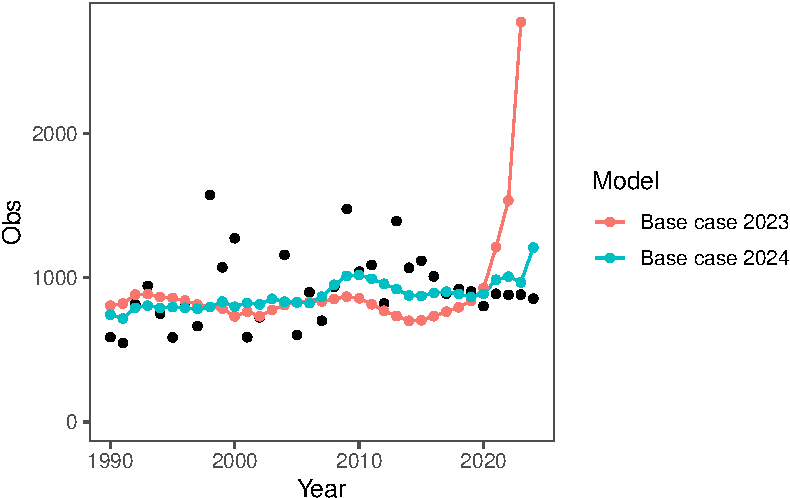
\includegraphics{00-Namibian_hake_model_2024_files/figure-pdf/fitidx1-1.pdf}

}

\caption{Base case model fits to main survey data compared to the
previous assessment.}

\end{figure}%

\begin{figure}[H]

{\centering 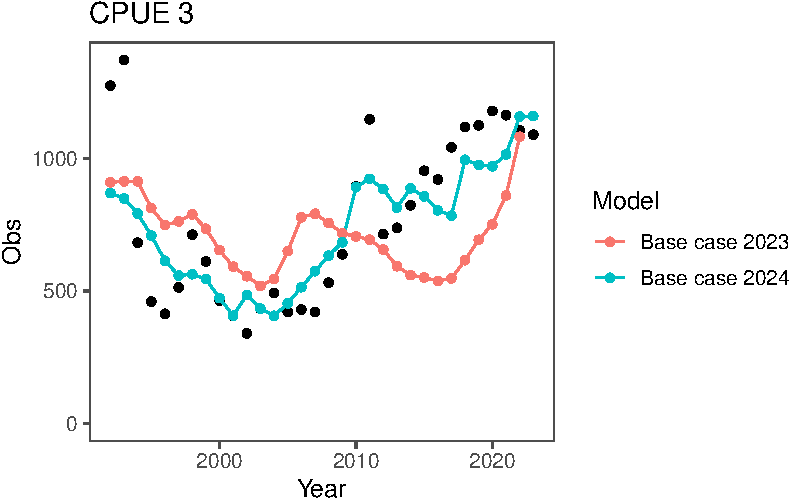
\includegraphics{00-Namibian_hake_model_2024_files/figure-pdf/fitcpue3-1.pdf}

}

\caption{Base case model fits to the CPUE index 3 data compared to the
previous assessment.}

\end{figure}%

\begin{Shaded}
\begin{Highlighting}[]
\NormalTok{dfcpue }\OtherTok{\textless{}{-}} \FunctionTok{rbind}\NormalTok{(}\FunctionTok{data.frame}\NormalTok{(}\AttributeTok{Year =} \DecValTok{1964}\SpecialCharTok{:}\DecValTok{2023}\NormalTok{, }\AttributeTok{Obs =}\NormalTok{ old\_bc}\SpecialCharTok{$}\NormalTok{Obs\_CPUE\_1, }\AttributeTok{predicted =}\NormalTok{ old\_bc}\SpecialCharTok{$}\NormalTok{e\_CPUE\_1,}
    \AttributeTok{Model =} \StringTok{"Base case 2023"}\NormalTok{), }\FunctionTok{data.frame}\NormalTok{(}\AttributeTok{Year =} \DecValTok{1964}\SpecialCharTok{:}\DecValTok{2024}\NormalTok{, }\AttributeTok{Obs =}\NormalTok{ m0}\SpecialCharTok{$}\NormalTok{Obs\_CPUE\_1,}
    \AttributeTok{predicted =}\NormalTok{ m0}\SpecialCharTok{$}\NormalTok{e\_CPUE\_1, }\AttributeTok{Model =} \StringTok{"Base case 2024"}\NormalTok{))}
\NormalTok{dfcpue }\SpecialCharTok{|\textgreater{}}
    \FunctionTok{filter}\NormalTok{(Obs }\SpecialCharTok{\textgreater{}} \DecValTok{0}\NormalTok{) }\SpecialCharTok{|\textgreater{}}
    \FunctionTok{ggplot}\NormalTok{(}\FunctionTok{aes}\NormalTok{(}\AttributeTok{x =}\NormalTok{ Year, }\AttributeTok{y =}\NormalTok{ Obs, }\AttributeTok{color =}\NormalTok{ Model)) }\SpecialCharTok{+} \FunctionTok{geom\_point}\NormalTok{(}\AttributeTok{color =} \StringTok{"black"}\NormalTok{) }\SpecialCharTok{+}
    \FunctionTok{geom\_line}\NormalTok{(}\FunctionTok{aes}\NormalTok{(}\AttributeTok{y =}\NormalTok{ predicted)) }\SpecialCharTok{+} \FunctionTok{geom\_point}\NormalTok{(}\FunctionTok{aes}\NormalTok{(}\AttributeTok{y =}\NormalTok{ predicted)) }\SpecialCharTok{+} \FunctionTok{ggtitle}\NormalTok{(}\StringTok{"CPUE 1"}\NormalTok{) }\SpecialCharTok{+}
    \FunctionTok{ylim}\NormalTok{(}\DecValTok{0}\NormalTok{, }\ConstantTok{NA}\NormalTok{)}
\end{Highlighting}
\end{Shaded}

\begin{figure}[H]

{\centering 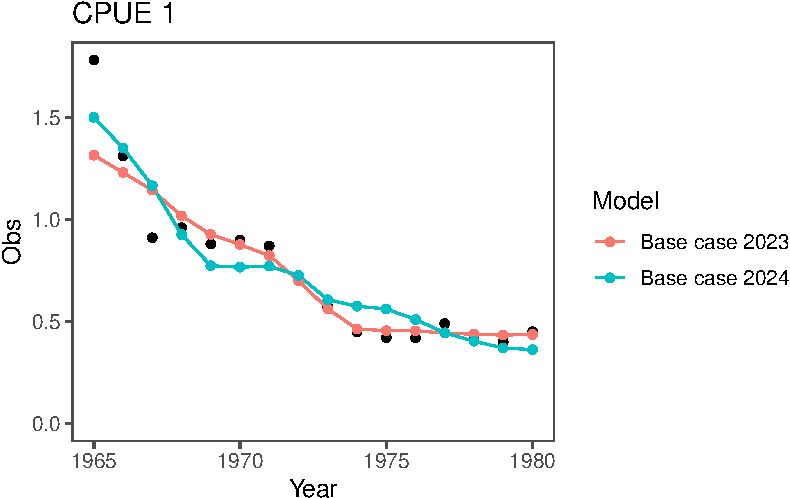
\includegraphics{00-Namibian_hake_model_2024_files/figure-pdf/fitcpue1-1.pdf}

}

\caption{Base case model fits to the CPUE index 1 data compared to the
previous assessment.}

\end{figure}%

\subsubsection{SSB results}\label{ssb-results}

\begin{figure}[H]

{\centering 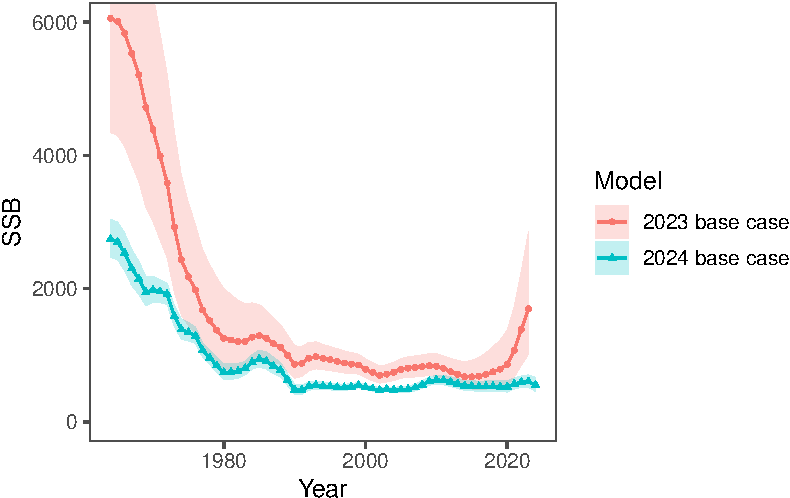
\includegraphics{00-Namibian_hake_model_2024_files/figure-pdf/fitssb-1.pdf}

}

\caption{Base case model showing the SSB estimates compared to the
previous assessment.}

\end{figure}%

\begin{Shaded}
\begin{Highlighting}[]
\NormalTok{mods }\SpecialCharTok{|\textgreater{}}
    \FunctionTok{filter}\NormalTok{(Model }\SpecialCharTok{\%in\%}\NormalTok{ mod\_label[}\DecValTok{1}\SpecialCharTok{:}\DecValTok{2}\NormalTok{], Year }\SpecialCharTok{\textgreater{}} \DecValTok{1960}\NormalTok{, Variable }\SpecialCharTok{==} \StringTok{"Depletion"}\NormalTok{) }\SpecialCharTok{|\textgreater{}}
    \FunctionTok{ggplot}\NormalTok{(}\FunctionTok{aes}\NormalTok{(}\AttributeTok{x =}\NormalTok{ Year, }\AttributeTok{y =}\NormalTok{ value, }\AttributeTok{ymin =}\NormalTok{ ymin, }\AttributeTok{ymax =}\NormalTok{ ymax, }\AttributeTok{type =}\NormalTok{ Model, }\AttributeTok{fill =}\NormalTok{ Model)) }\SpecialCharTok{+}
    \FunctionTok{geom\_ribbon}\NormalTok{(}\AttributeTok{alpha =} \FloatTok{0.24}\NormalTok{) }\SpecialCharTok{+}\NormalTok{ ggthemes}\SpecialCharTok{::}\FunctionTok{theme\_few}\NormalTok{() }\SpecialCharTok{+} \FunctionTok{geom\_line}\NormalTok{(}\FunctionTok{aes}\NormalTok{(}\AttributeTok{color =}\NormalTok{ Model)) }\SpecialCharTok{+}
    \FunctionTok{geom\_point}\NormalTok{(}\FunctionTok{aes}\NormalTok{(}\AttributeTok{color =}\NormalTok{ Model, }\AttributeTok{shape =}\NormalTok{ Model), }\AttributeTok{size =} \DecValTok{1}\NormalTok{) }\SpecialCharTok{+} \FunctionTok{ylab}\NormalTok{(}\StringTok{"Relative SSB"}\NormalTok{) }\SpecialCharTok{+}
    \FunctionTok{xlab}\NormalTok{(}\StringTok{"Year"}\NormalTok{)}
\end{Highlighting}
\end{Shaded}

\begin{figure}[H]

{\centering 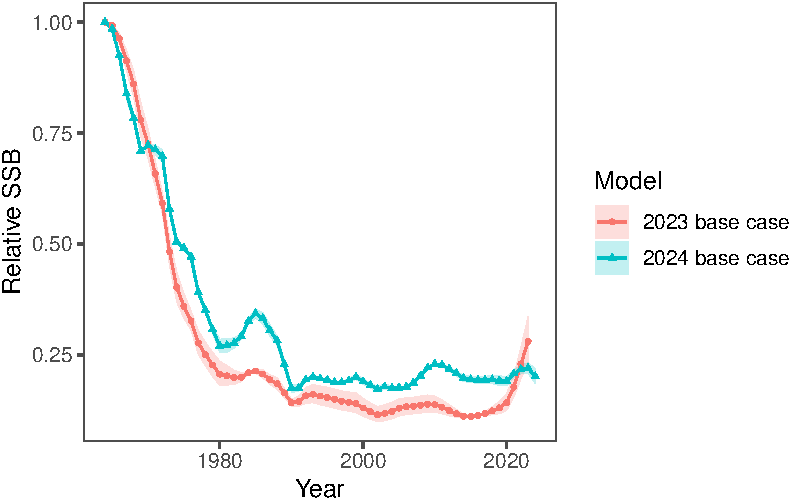
\includegraphics{00-Namibian_hake_model_2024_files/figure-pdf/depl-1.pdf}

}

\caption{Base case model showing the relative SSB estimates compared to
the previous assessment.}

\end{figure}%

\begin{figure}[H]

{\centering 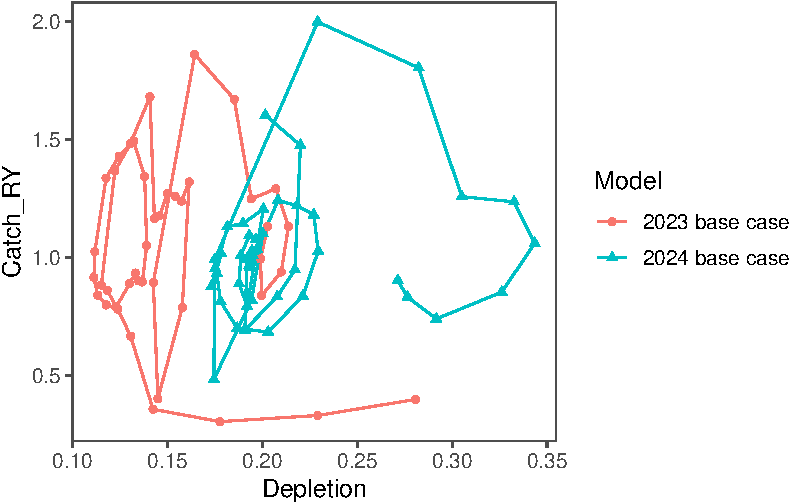
\includegraphics{00-Namibian_hake_model_2024_files/figure-pdf/kobe-1.pdf}

}

\caption{Base case model showing the relative SSB estimates compared to
the previous assessment.}

\end{figure}%

\begin{figure}[H]

{\centering 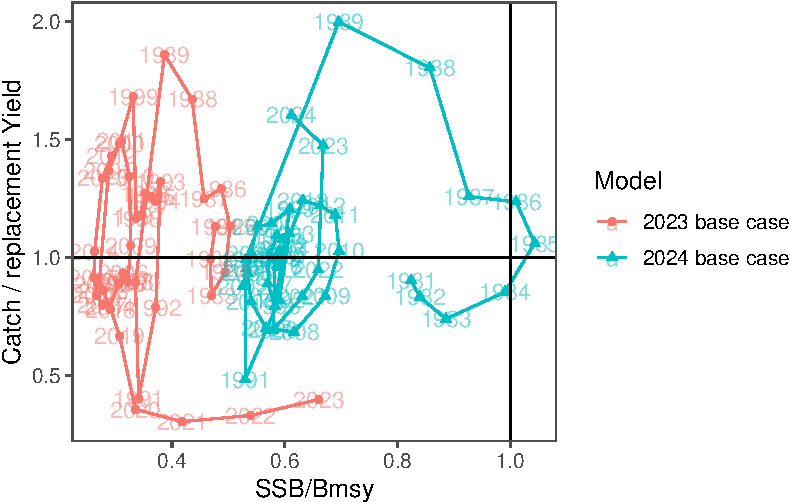
\includegraphics{00-Namibian_hake_model_2024_files/figure-pdf/kobe-2.pdf}

}

\caption{Base case model showing the relative SSB estimates compared to
the previous assessment.}

\end{figure}%

\begin{figure}[H]

{\centering 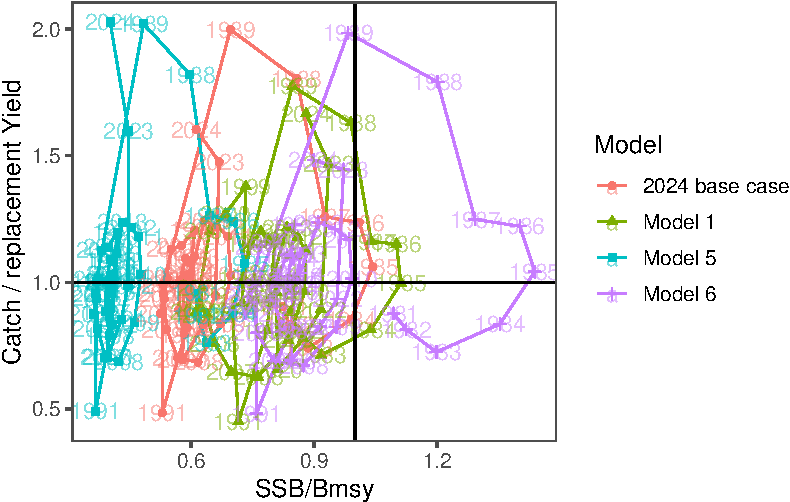
\includegraphics{00-Namibian_hake_model_2024_files/figure-pdf/kobe-3.pdf}

}

\caption{Base case model showing the relative SSB estimates compared to
the previous assessment.}

\end{figure}%

\subsubsection{Age composition fits}\label{age-composition-fits}

\begin{figure}[H]

{\centering 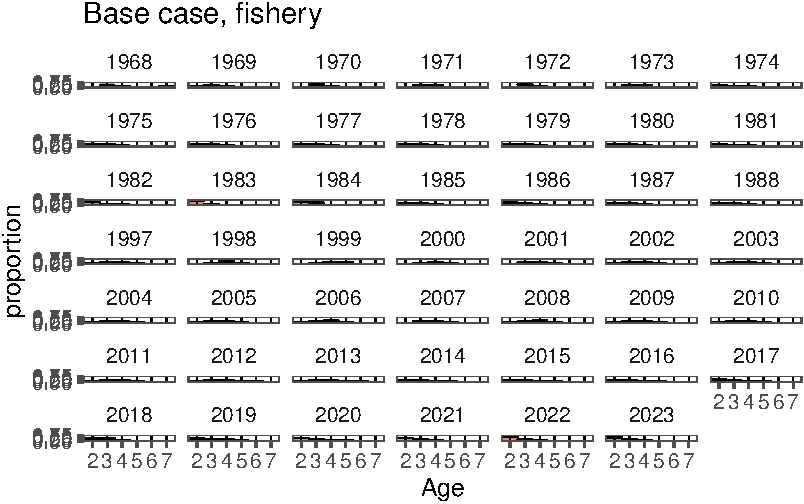
\includegraphics{00-Namibian_hake_model_2024_files/figure-pdf/agecomps-1.pdf}

}

\caption{Base case model fits to survey and fishery age composition
data. Note that the base case model uses a `minus group' equal to `1'
for the survey data.}

\end{figure}%

\begin{figure}[H]

{\centering 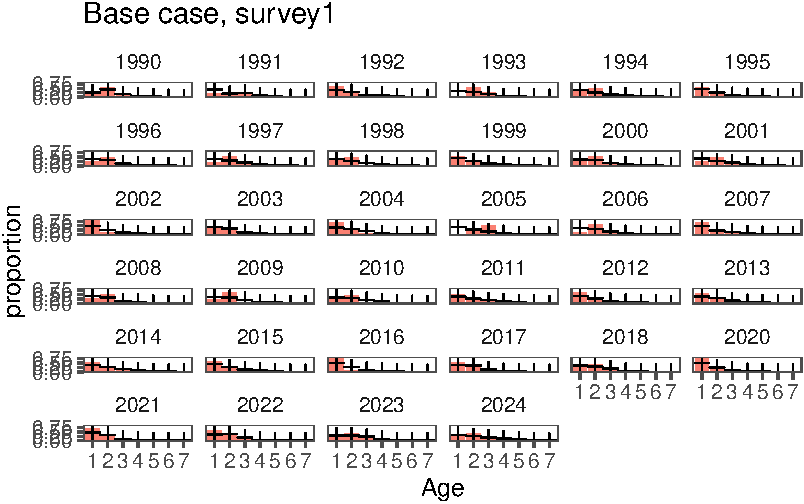
\includegraphics{00-Namibian_hake_model_2024_files/figure-pdf/agecomps-2.pdf}

}

\caption{Base case model fits to survey and fishery age composition
data. Note that the base case model uses a `minus group' equal to `1'
for the survey data.}

\end{figure}%

\subsubsection{Selectivity}\label{selectivity}

\begin{figure}[H]

{\centering 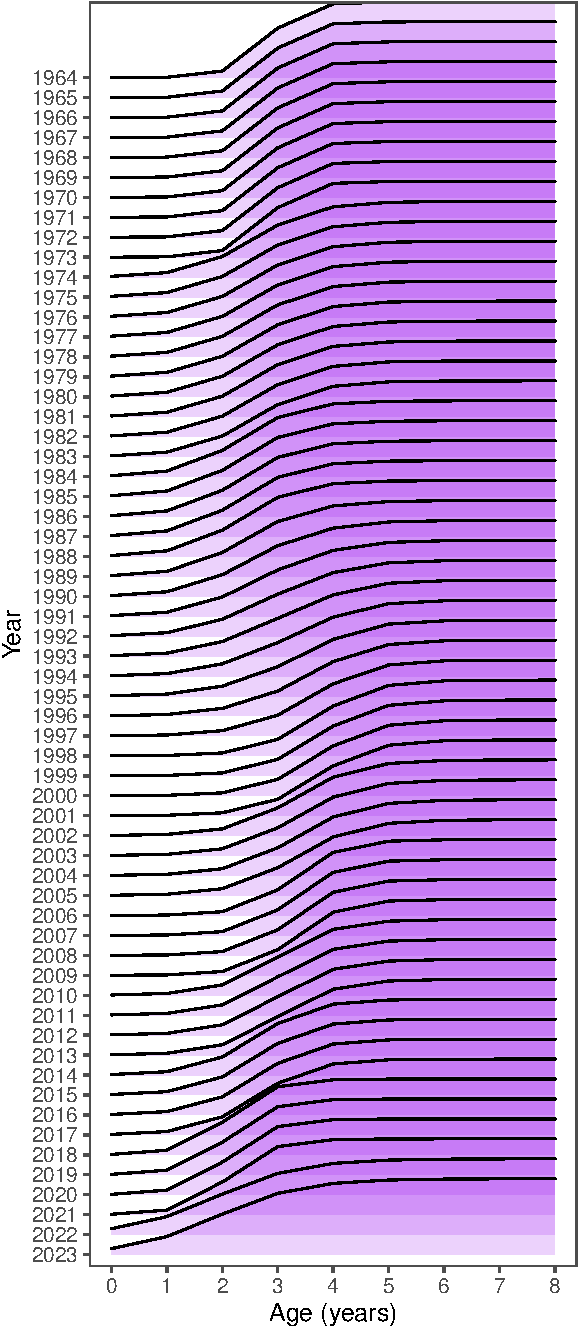
\includegraphics{00-Namibian_hake_model_2024_files/figure-pdf/selex-1.pdf}

}

\caption{Selectivity estimates for the base-case model run.}

\end{figure}%

\subsubsection{Stock-recruitment curves}\label{stock-recruitment-curves}

The following plot shows the stock-recruitment curves for the base case
and models 1, 2, 3, and 5 and 6.

\begin{verbatim}
   Warning: The shape palette can deal with a maximum of 6 discrete values because more
   than 6 becomes difficult to discriminate
   i you have requested 8 values. Consider specifying shapes manually if you need
     that many have them.
   Warning: Removed 40 rows containing missing values or values outside the scale range
   (`geom_point()`).
\end{verbatim}

\begin{figure}[H]

{\centering 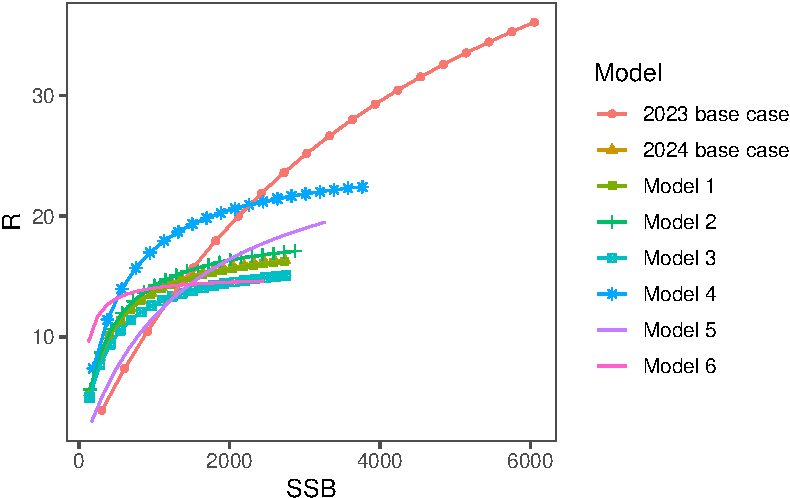
\includegraphics{00-Namibian_hake_model_2024_files/figure-pdf/srrplots-1.pdf}

}

\caption{Model runs}

\end{figure}%

\subsubsection{Stock status comparisons}\label{stock-status-comparisons}

Unclear why this table doesn't show up\ldots{}

\begin{Shaded}
\begin{Highlighting}[]
\NormalTok{dftmp }\OtherTok{\textless{}{-}} \ConstantTok{NULL}
\NormalTok{mod\_scen }\OtherTok{\textless{}{-}} \FunctionTok{c}\NormalTok{(}\DecValTok{2}\SpecialCharTok{:}\DecValTok{5}\NormalTok{)}
\ControlFlowTok{for}\NormalTok{ (ii }\ControlFlowTok{in}\NormalTok{ mod\_scen) \{}
\NormalTok{    x }\OtherTok{\textless{}{-}}\NormalTok{ modlst[[ii]]}
    \StringTok{"{-}ln(Likelihood)"}
\NormalTok{    nll }\OtherTok{\textless{}{-}}\NormalTok{ x}\SpecialCharTok{$}\NormalTok{ObjFun}
    \FunctionTok{names}\NormalTok{(nll) }\OtherTok{\textless{}{-}} \StringTok{"Overall"}
\NormalTok{    CPUE }\OtherTok{\textless{}{-}}\NormalTok{ x}\SpecialCharTok{$}\NormalTok{CPUE\_Like}
    \FunctionTok{names}\NormalTok{(CPUE) }\OtherTok{\textless{}{-}} \StringTok{"CPUE"}
\NormalTok{    surv }\OtherTok{\textless{}{-}}\NormalTok{ x}\SpecialCharTok{$}\NormalTok{Survey\_Like}
    \FunctionTok{names}\NormalTok{(surv) }\OtherTok{\textless{}{-}} \StringTok{"Survey"}
\NormalTok{    caa }\OtherTok{\textless{}{-}}\NormalTok{ x}\SpecialCharTok{$}\NormalTok{CAA\_Likelihood}
    \FunctionTok{names}\NormalTok{(caa) }\OtherTok{\textless{}{-}} \StringTok{"Commercial CAA"}
\NormalTok{    caas }\OtherTok{\textless{}{-}}\NormalTok{ x}\SpecialCharTok{$}\NormalTok{CAAS\_Likelihood}
    \FunctionTok{names}\NormalTok{(caas) }\OtherTok{\textless{}{-}} \StringTok{"Survey CAA"}
\NormalTok{    rec }\OtherTok{\textless{}{-}}\NormalTok{ x}\SpecialCharTok{$}\NormalTok{RecRes\_Likelihood}
    \FunctionTok{names}\NormalTok{(x}\SpecialCharTok{$}\NormalTok{RecRes\_Likelihood) }\OtherTok{\textless{}{-}} \StringTok{"Recruitment Residuals"}
\NormalTok{    oneyrold }\OtherTok{\textless{}{-}}\NormalTok{ x}\SpecialCharTok{$}\NormalTok{Oneyearold\_Likelihood}
    \FunctionTok{names}\NormalTok{(oneyrold) }\OtherTok{\textless{}{-}} \StringTok{"One year old Biomass"}
\NormalTok{    NumPars }\OtherTok{\textless{}{-}}\NormalTok{ x}\SpecialCharTok{$}\NormalTok{Npars}
    \FunctionTok{names}\NormalTok{(NumPars) }\OtherTok{\textless{}{-}} \StringTok{"Number of parameters estimated"}
\NormalTok{    AIC }\OtherTok{\textless{}{-}}\NormalTok{ x}\SpecialCharTok{$}\NormalTok{Akaike}
    \FunctionTok{names}\NormalTok{(AIC) }\OtherTok{\textless{}{-}} \StringTok{"AIC"}

\NormalTok{    v }\OtherTok{\textless{}{-}} \FunctionTok{c}\NormalTok{(nll, CPUE, surv, caa, caas, rec, oneyrold, NumPars, AIC)}
\NormalTok{    dftmp }\OtherTok{\textless{}{-}} \FunctionTok{cbind}\NormalTok{(dftmp, v)}
\NormalTok{\}}
\NormalTok{dftmp }\OtherTok{\textless{}{-}} \FunctionTok{data.frame}\NormalTok{(}\FunctionTok{rownames}\NormalTok{(dftmp), dftmp, }\AttributeTok{row.names =} \ConstantTok{NULL}\NormalTok{)}
\FunctionTok{names}\NormalTok{(dftmp) }\OtherTok{\textless{}{-}} \FunctionTok{c}\NormalTok{(}\StringTok{"Component"}\NormalTok{, mod\_label[mod\_scen])}
\NormalTok{tabcap }\OtherTok{\textless{}{-}} \StringTok{"Model fits to data components"}
\NormalTok{tab }\OtherTok{\textless{}{-}} \FunctionTok{xtable}\NormalTok{(dftmp, }\AttributeTok{caption =}\NormalTok{ tabcap, }\AttributeTok{type =} \StringTok{"html"}\NormalTok{, }\AttributeTok{label =} \StringTok{"tab:mgt\_quants"}\NormalTok{, }\AttributeTok{digits =} \DecValTok{3}\NormalTok{)}
\CommentTok{\# align=paste0(\textquotesingle{}lll\textquotesingle{},strrep(\textquotesingle{}r\textquotesingle{},length(mod\_scen+1))))}
\FunctionTok{print}\NormalTok{(tab, }\AttributeTok{caption.placement =} \StringTok{"top"}\NormalTok{, }\AttributeTok{include.rownames =} \ConstantTok{FALSE}\NormalTok{, }\AttributeTok{sanitize.text.function =} \ControlFlowTok{function}\NormalTok{(x) \{}
\NormalTok{    x}
\NormalTok{\})}
\end{Highlighting}
\end{Shaded}

\% latex table generated in R 4.4.1 by xtable 1.8-4 package \% Tue Jul
16 09:28:51 2024

\begin{table}[ht]
\centering
\caption{Model fits to data components} 

\begin{tabular}{lrrrr}
  \hline
Component & 2024 base case & Model 1 & Model 2 & Model 3 \\ 
  \hline
Overall & -2.321 & 14.367 & 68.658 & -2.366 \\ 
  CPUE & -48.020 & -49.299 & -46.101 & -47.800 \\ 
  Survey & -32.623 & -21.843 & -19.284 & -32.825 \\ 
  Commercial CAA & -105.569 & -94.865 & -53.299 & -105.279 \\ 
  Survey CAA & 116.190 & 117.910 & 141.296 & 117.055 \\ 
   & 28.660 & 27.597 & 18.453 & 27.992 \\ 
  One year old Biomass & 70.009 & 70.569 & 73.385 & 69.853 \\ 
  Number of parameters estimated & 83.000 & 83.000 & 83.000 & 84.000 \\ 
  AIC & 161.358 & 194.735 & 303.317 & 163.268 \\ 
   \hline
\end{tabular}
\end{table}

But here the figure does\ldots{} \#\textbar{} \# x\(KspSTD
# x\)KexpSTD\\
\# Ksp \# h \# Bsp(2023) \# Bexp(2023) \# Bsp(2023)/Ksp \# Bsp(2024) \#
Bexp(2024) \# Bsp(2024)/Ksp \# Bspmsy \# Bspmsy/Ksp \# Bsp(2023)/Bspmsy
\# Bsp(2024)/Bspmsy \# MSY \# AverageRY\_5yrs \#
AverageRY\_5yrs*Bsp/Bspmsy \# ```\{r mgt\_quants, results = ``asis''\}
\# Mgt quants by model

\begin{figure}[H]

{\centering 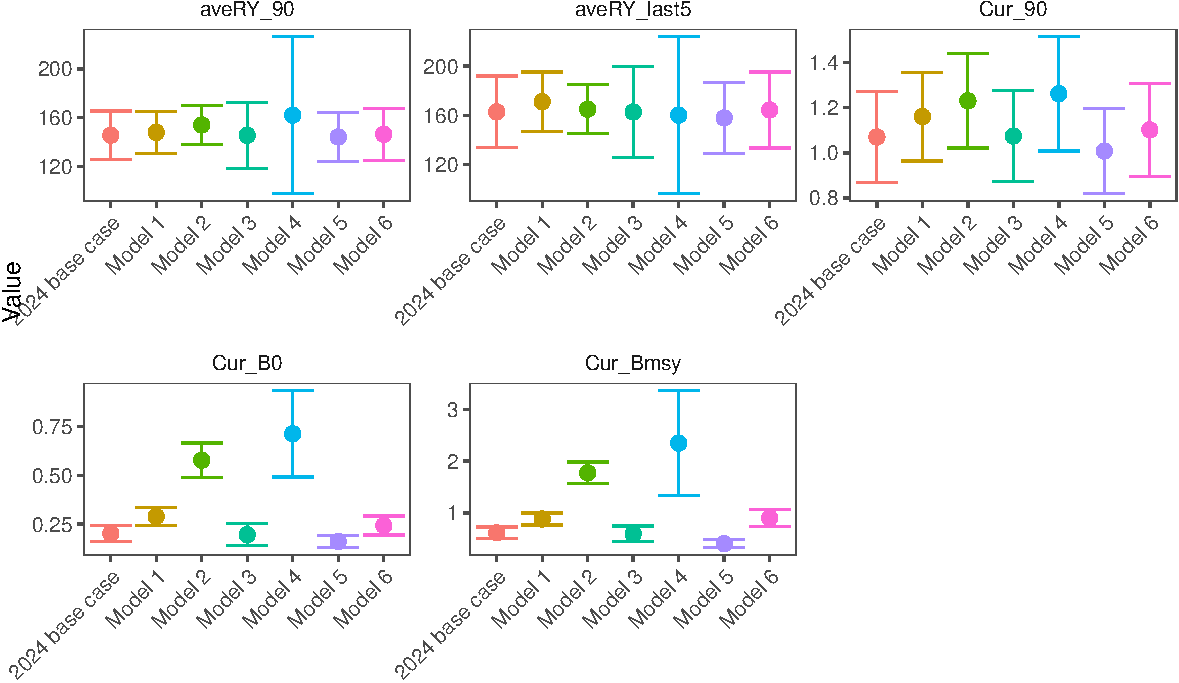
\includegraphics{00-Namibian_hake_model_2024_files/figure-pdf/stockstatus-1.pdf}

}

\caption{Some reference point comparisons among model runs. aveRY\_90 is
the average replacement yeild since 1990, aveRY is the average
replacement yield over the most recent 5 years before the current year,
Cur\_90 is the current (terminal year) SSB over the estimate from 1990,
Cur\_B0 is over the unfished estimate, and Cur\_Bmsy is the ratio of
current SSB over the Bmsy estimate.}

\end{figure}%

\section{Control rule application}\label{control-rule-application}

\subsection{Design of triggered control
rule}\label{design-of-triggered-control-rule}

The situation for developing a two-species control rule where catches
between species and the trend in overall biomass for both species is
combined is challenging. For management purposes, the goal is to avoid
incidental takes in the proportion of one species that exceeds the
historical levels of depletion for either stock. Fortunately, survey
data are available that can be used to distinguish trends in the
relative biomass for both stocks. The design of the triggered control
rule therefore must consider patterns in the relative biomass from the
survey data, the absolute biomass of the combined catch and biomass as
modeled from the combined-stocks assessment. This provides a pragmatic
approach using available data.

The steps in the control rule would be first to run a simple model that
projected the survey biomass and relative proportion of \emph{M.
paradoxus}. Then, given the mean proportion over the period, compute the
adjustment needed to the overarching control rule for the management
procedure. For example, the historical range based on the survey has
been between about one third of the mean value (in the earliest part of
the period) to about 70\% above the mean proportion. This range
(especially the lower value) was used as a semi-empirical way to develop
a minimum stock size threshold as part of the control rule. That is,
when the stock of \emph{M. paradoxus} drops below 30\% of the mean
proportion of the combined stocks estimate, the TAC recommendation for
the combined stock would be zero. So if proportion of \emph{M.
paradoxus} \((p_y)\) is greater than 30\% of the long-term mean
proportion, then

\(TAC_y=(0.8 \sum_{y}^{y-4}\frac{RY_y} 5) \min(1,B_y/B_{MSY})  \min(1,p_y/\bar{p})\)

In words, the TAC in year y is equal to the catch under the current
control rule times the ratio of the spawning biomass relative to BMSY
(or proxy) and the externally estimated proportion of \emph{M.
paradoxus} from survey data. The second and third terms on the right
hands side are depicted in Table 1 (and include the zero catch
recommended if the \emph{M. paradoxus} proportion dropped below the
lowest value historically observed). The values of γ,λ were both set to
1.0 but could be adjusted (say to 0.5) to have a more gradual transition
as the proportion or aggregate stock conditions drop below mean levels.
We note that the specification of a survey linkage by the individual
species provides a trigger (30\% of long-term mean) that reduces the
exploitation rate as the point of recruitment impairment (PRI) is
approached.

Improvements to this approach could benefit from management that
accounts for the depth of fishing Johnsen and Kathena (2012). These data
were unavailable for inclusion in this study since they rely on
predictions of the species mix based on the depth of fishing. Also, it
is unclear that depth of fishing could be forecasted in a manner that
could be built into a management measure.

The approached applied a smoother to each of the species time-series of
survey data.

\subsection{Modeling Namibian hake survey data by
species}\label{modeling-namibian-hake-survey-data-by-species}

Fisheries stock assessments require data that are reliably collected and
compiled. Secondarily, assessment models should be configured to match
the assumptions associated with the observed data. To account for survey
trends between the two species of hake we applied the estimated
observation errors to a simple state-space random walk model. This
approach has a number of options for how process-errors can be specified
and estimated. The observation model applies the observation-error
variances \((σ_(j,t)^2)\) for the \(j^{th}\) species in year
\(t (x_(j,t) )\). The indices are fit to latent state variables, e.g.,
the underlying population trend \(ln(Z ̂_(j,t )\) as follows:

\(ln(Z_(j,t) ) = ln(Z ̂_(j,t) )+ϵ_(j,t),"where " ϵ_(j,t)∼N(0,σ_(j,t)^2 )\)

and the state equation and associated process error variance σ\_PE\^{}2
is defined as

\(ln(Z ̂_(j,t+1) )=ln(Z ̂_(j,t) )+η_(j,t),"where " η_(j,t)∼N(0,τ_j^2 ).\)

The process error variances τ\_j\^{}2 (which may or may not vary across
indices) are fixed effect parameters and the unobserved species combined
population ln(Z\_(j,t) ) is estimated as a series of random effects. The
model is fit using maximum likelihood estimation in TMB using the R
package ``rema'' (Sullivan 2022). The survey data for each species was
used with CVs applied for observation error specifications. The values
for τ\_j\^{}2 were estimated for each species since their inherent
variability may differ.

The above analysis provides a summary of the model runs and the design
of a control rule that accounts for the signals in the data on the
different species.

\section{Notes}\label{notes}

Throughout the weeks, we scrutinized data inputs and found a couple of
inconsistencies. For example, data were provided for surveys in 2019 yet
there were no observations in that year. Similarly, the
abundance-at-length data from the surveys failed to identify strong
periods of persistence by cohorts.

Ignore 7-vessel CPUE data set.



\end{document}
